%tp1_topo.tex

\section{Topologie du R\'eseau}

Le r\'eseau simul\'e est compos\'e de deux sites avec un lien du premier vers le second
d'une capacit\'e de 2Mb/s et de latence 20ms.
Sa file d'attente de type {\em DropTail} peut supporter 100 paquets.

Quatre trafics sont mis en place :
\begin{itemize}
	\item la premi\`ere connexion suit le protocole UDP, son d\'ebit est exponentiel, la
	dur\'ee moyenne des p\'eriodes d'activit\'e est de 10ms, tandis que celles
	d'inactivit\'e durent 5 ms ;
	\item les trois autres suivent un protocole TCP, et sont de d\'ebits constants, leurs
	latences respectives sont de 50ms, 100ms et 150ms.
\end{itemize}

Le débit moyen théorique de chacune de ces connexions est de 1Mb/s, il était donc
nécessaire de calculer le débit crête du lien UDP de manière à pouvoir obtenir un débit
moyen théorique juste malgré les périodes d'inactivité.\\
$\bar{\lambda} = \frac{\lambda_{crete} \times ON}{ON + OFF}$\\
On a donc : $\lambda_{crete} = \frac{(ON + OFF) \times \bar{\lambda}}{ON}$.\\
On en déduit $\lambda_{crete} = 1.5 Mb/s$.

De plus il fallait également calculer la taille des paquets des connexions TCP de manière
à assurer le débit moyen théorique de 1Mb/s.\\
$\bar{\lambda} = \frac{taille_paquet}{intervalle}$\\
On a donc : $taille_paquet = \bar{\lambda} \times intervalle$.\\
Les tailles de paquets sont donc respectivement :
\begin{itemize}
	\item 6250 octets,
	\item 12500 octets,
	\item 18750 octets.
\end{itemize}

Les quatre connexions sont lancées simultanément au démarrage, et sont stoppées à 10
secondes du démarrage.

\hbox{
	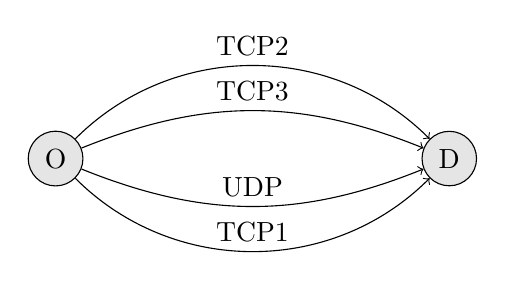
\begin{tikzpicture}
		\node[circle,draw,fill=black!10] (O) at (0,0) {O};
		\node[circle,draw,fill=black!10] (D) at (5,0) {D}
			edge[<-,bend left=22] node[above] {UDP} (O)
			edge[<-,bend left=45] node[above] {TCP1} (O)
			edge[<-,bend right=45] node[above] {TCP2} (O)
			edge[<-,bend right=22] node[above] {TCP3} (O)
			;
	\end{tikzpicture}
%\caption{Topologie}
\label{topo_fig}
}

